\documentclass[tikz,border=8pt]{standalone}
\usetikzlibrary{arrows.meta,positioning}
\begin{document}
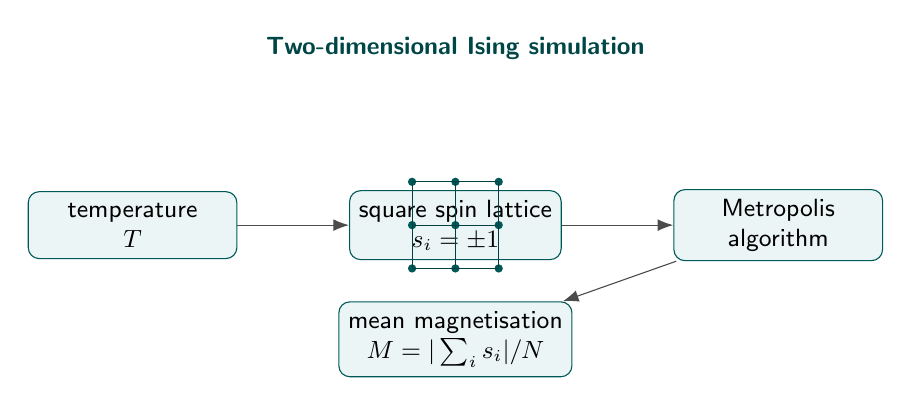
\begin{tikzpicture}[box/.style={draw=teal!70!black,fill=teal!8,rounded corners,minimum width=2.65cm,minimum height=.85cm,align=center,font=\sffamily\small},a/.style={-{Latex[length=2mm]},draw=black!70}]
\node[font=\sffamily\bfseries\small,text=teal!55!black] at (0,2.25) {Two-dimensional Ising simulation};
\node[box] (temp) at (-4.1,0) {temperature\\$T$};
\node[box] (lattice) at (0,0) {square spin lattice\\$s_i=\pm1$};
\node[box] (mc) at (4.1,0) {Metropolis\\algorithm};
\draw[a] (temp)--(lattice); \draw[a] (lattice)--(mc);
\node[box] (obs) at (0,-1.45) {mean magnetisation\\$M=|\sum_i s_i|/N$};
\draw[a] (mc)--(obs);
\foreach \x in {-0.55,0,0.55} {\foreach \y in {-0.55,0,0.55} {\fill[teal!70!black] (\x,\y) circle (1.5pt);}}
\draw[teal!50!black] (-.55,-.55) grid[step=.55] (.55,.55);
\end{tikzpicture}
\end{document}
